
\chapter{Introduction}

%In large companies, it is possible to have dozens or even hundreds of software projects underway at any given point in time. This kind of scale produces new challenges, as well as new opportunities for these companies. Both challenges and opportunities result from the need of the company to successfully understand and exploit their ownership of a portfolio of software projects. 

%Single project management is easy to achieve from various way. Many software metrics, such as coverage, complexity and file size, provide significant information about a software project. But it is reported that, almost all metrics have deficiency when judge a state of a project with only one or two of them. Therefore, people usually trend to look into more metrics to understand a project. However, while the number of projects increases as well as the number of metrics increases, the data to read inflates rapidly and become overwhelming.

%In order to address this issue and achieve efficient governance over large number of projects, we introduce an analysis tool called Software Intensive Care Unit. It is from the idea of intensive care unit in hospitals where patients are placed with sensors from sophisticated machines and they are consistently monitoring the patients' various vital sign such as pulse, breathe, etc. Similarly, Software Intensive Care Unit(SICU) provides various software metrics, each of which reveals one aspect of the project. These metrics are the vital signs of a software project. With all these vital signs together, users can have a fast but complete view of the projects, leading to easier understanding of projects and make better decisions and practice. Though one might argue that software projects' performance cannot be simply judged by a set of metrics, the case is the same in medicine. A doctor will not simply diagnose a patient by those vital signs, but it is undoubtedly that the medical intensive care unit helps the diagnosis a lot, so it is the software intensive care unit.

%However, to build up the SICU is a great challenge. Both what data to show and how to show them are essential to successfully set up a SICU that offer enough insight into the most interesting aspect of the projects without too much data overwhelming. Moreover, interesting things are various from different situation. Some setting may be common over projects and organization, but we don't believe there is a golden rule for all projects. So system should give users the capability to customize as their need.
This paper

\section{The Problem}
In most of the software project development cases, software metrics are one of the essential tools for performance measuring and quality control. But they are not comprehensive enough to make judgement with only one or two. So, we need to utilize multiple metrics in order to acquire insight of the health state of the software project. The more software metrics we look into, the more comprehensive insight we will get, but also the more effort it will need to collect measure data and interpret metrics values. My research tries to overcome this challenge by developing a system to help observer the health state of the software project from multiple software metrics in an effective way.

\section{Software Intensive Care Unit Approach}
What is SICU

\section{Thesis Claim}
We claim it is the most powerful tool ever in the world! =P

\section{Evaluation}
We evaluate in a classroom.

\section{Thesis Structure}
Here is a paragraph that saying the same thing as TOC.

\chapter{Related Work}
This chapter presents some related work of my research. Four parts of relative work will be discussed in the chapter.

First part discusses previous research of empirical software engineering concepts. Most of previous research of measurement-based software engineering are focus on the methodology. Effective approaches are developed and deployed to actual practice. Research of Hackystat and Software ICU is towards the 3rd generation of approaches to PSP metrics\cite{csdl2-02-07}.

Second part discusses three recent researches that focus on automated data collection. Two of them mainly focus on introduction level programming course and lack of system extensibility, which means no use to senior software development or professional settings. The third one is very similar to Hackystat.

Third part discusses some commercial ``dashboards'' for software project data. Software ICU is, of course, one example of a project dashboard. However, it differs from commercial approaches with its intensive metrics, high extensibility and open source development and distribution. 

Four part discusses two previous case studies of Hackystat system. This is the third case study of Hackystat system. So I will discuss the two related previous studies to provide some insight into the development history of Hackystat.

\section {TSP/PSP}
The Personal Software Process(PSP)\cite{book:psp} and the Team Software Process(TSP)\cite{book:tsp} are among the most extensively studied approaches for measurement-based software engineering. They were developed by Watts Humphrey to teach students (in university and industry alike) to the use of large scale methods based on the Capability Maturity Model (CMM). It scales down industrial software practices to fit the needs of small scale program development. Software processes and software engineering disciplines are gradually introduced through small program projects (e.g. course assignment projects). The PSP maturity progression is shown in \autoref{fig:PSP-Evo}. Students gather both process and product measures of each involved projects. By comparing the measurement result to their original planning, they understand their programming habits, both pros and cons, and refine their process to higher level of maturity level.

\begin{figure}[htbp] %  figure placement: here, top, bottom, or page
   \centering
   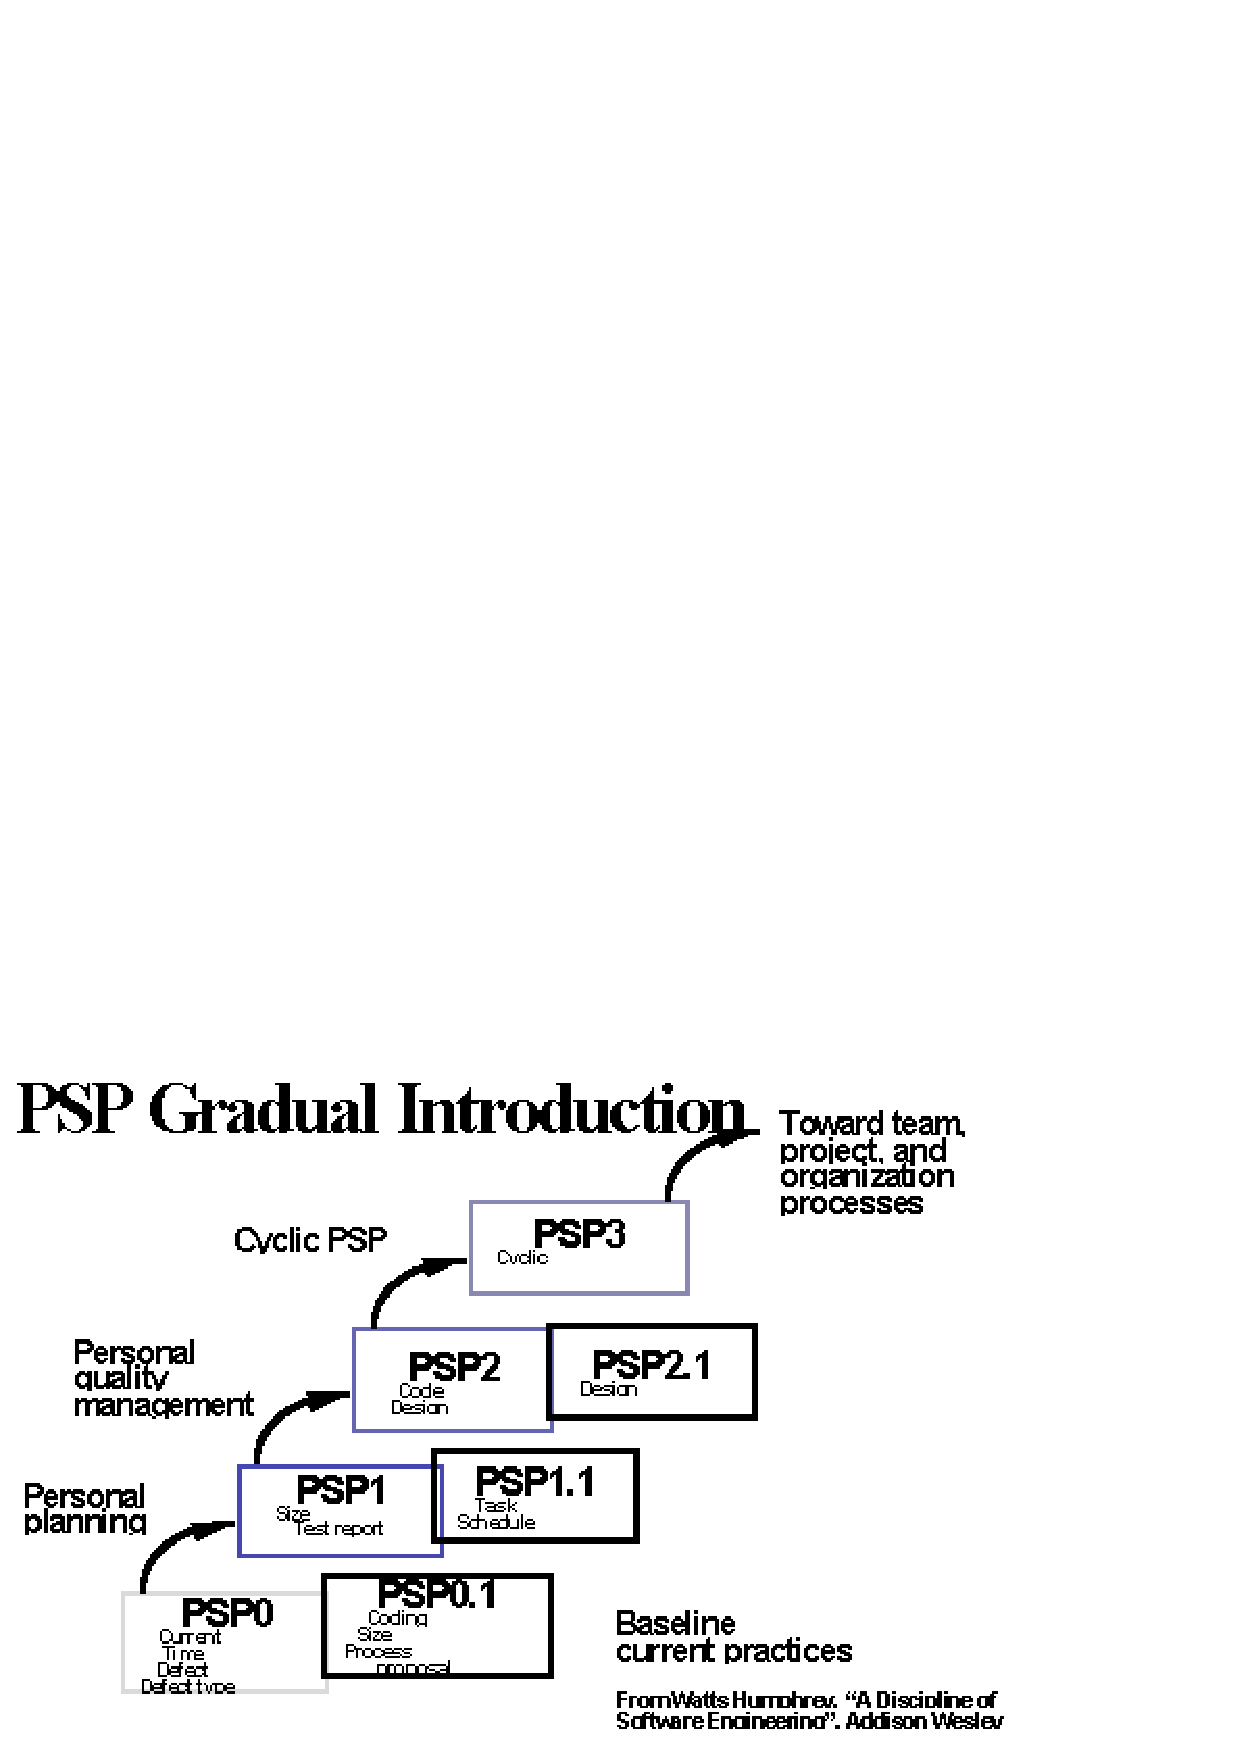
\includegraphics[height=20em]{PSP-Evo} 
   \caption{Progression of PSP}
   \label{fig:PSP-Evo}
\end{figure}

PSP/TSP is proven to be effective on both academic education as well as industrial application. (more about related research)

Its major drawback is the lack of automation. Developers have to manually record their process and product data (mostly the development time and number of defects). The high overhead of data collection holds a barrier to its introduction and adoption. Additionally, it is not easy to ``digest'' the data. developers have to manually analyze their logged data in order to understand the defect of their performance, then be able to improve it.

On the contrary, Software ICU provide a much higher level of automation in tracking and analyzing software process and product data.


\section {Research Based on Automated Data Collection}
Project ClockIt and Retina are two recent researches based on automated data collection to support entry-level programming courses, while PROM is the most similar research to Hackystat.

Project ClockIt provides a data logger as BlueJ\footnote{``BlueJ is an integrated Java environment specifically designed for introductory teaching.'' --Quoted from \url{http://www.bluej.org/about/what.html}}
 extension. It logs user's open/close of project and package, file change and delete and compilation results. Data is logged to local file and later send to a database via internet. An data visualizer integrated to BlueJ is available to view data about the current project. \autoref{fig:clockit} shows an example of this visualizer. Data stored in their database is used for statistic analysis such as class averages. A web interface is also available to instructors to view the individual data of their students and class average analysis data.

\begin{figure}[htbp] %  figure placement: here, top, bottom, or page
   \centering
   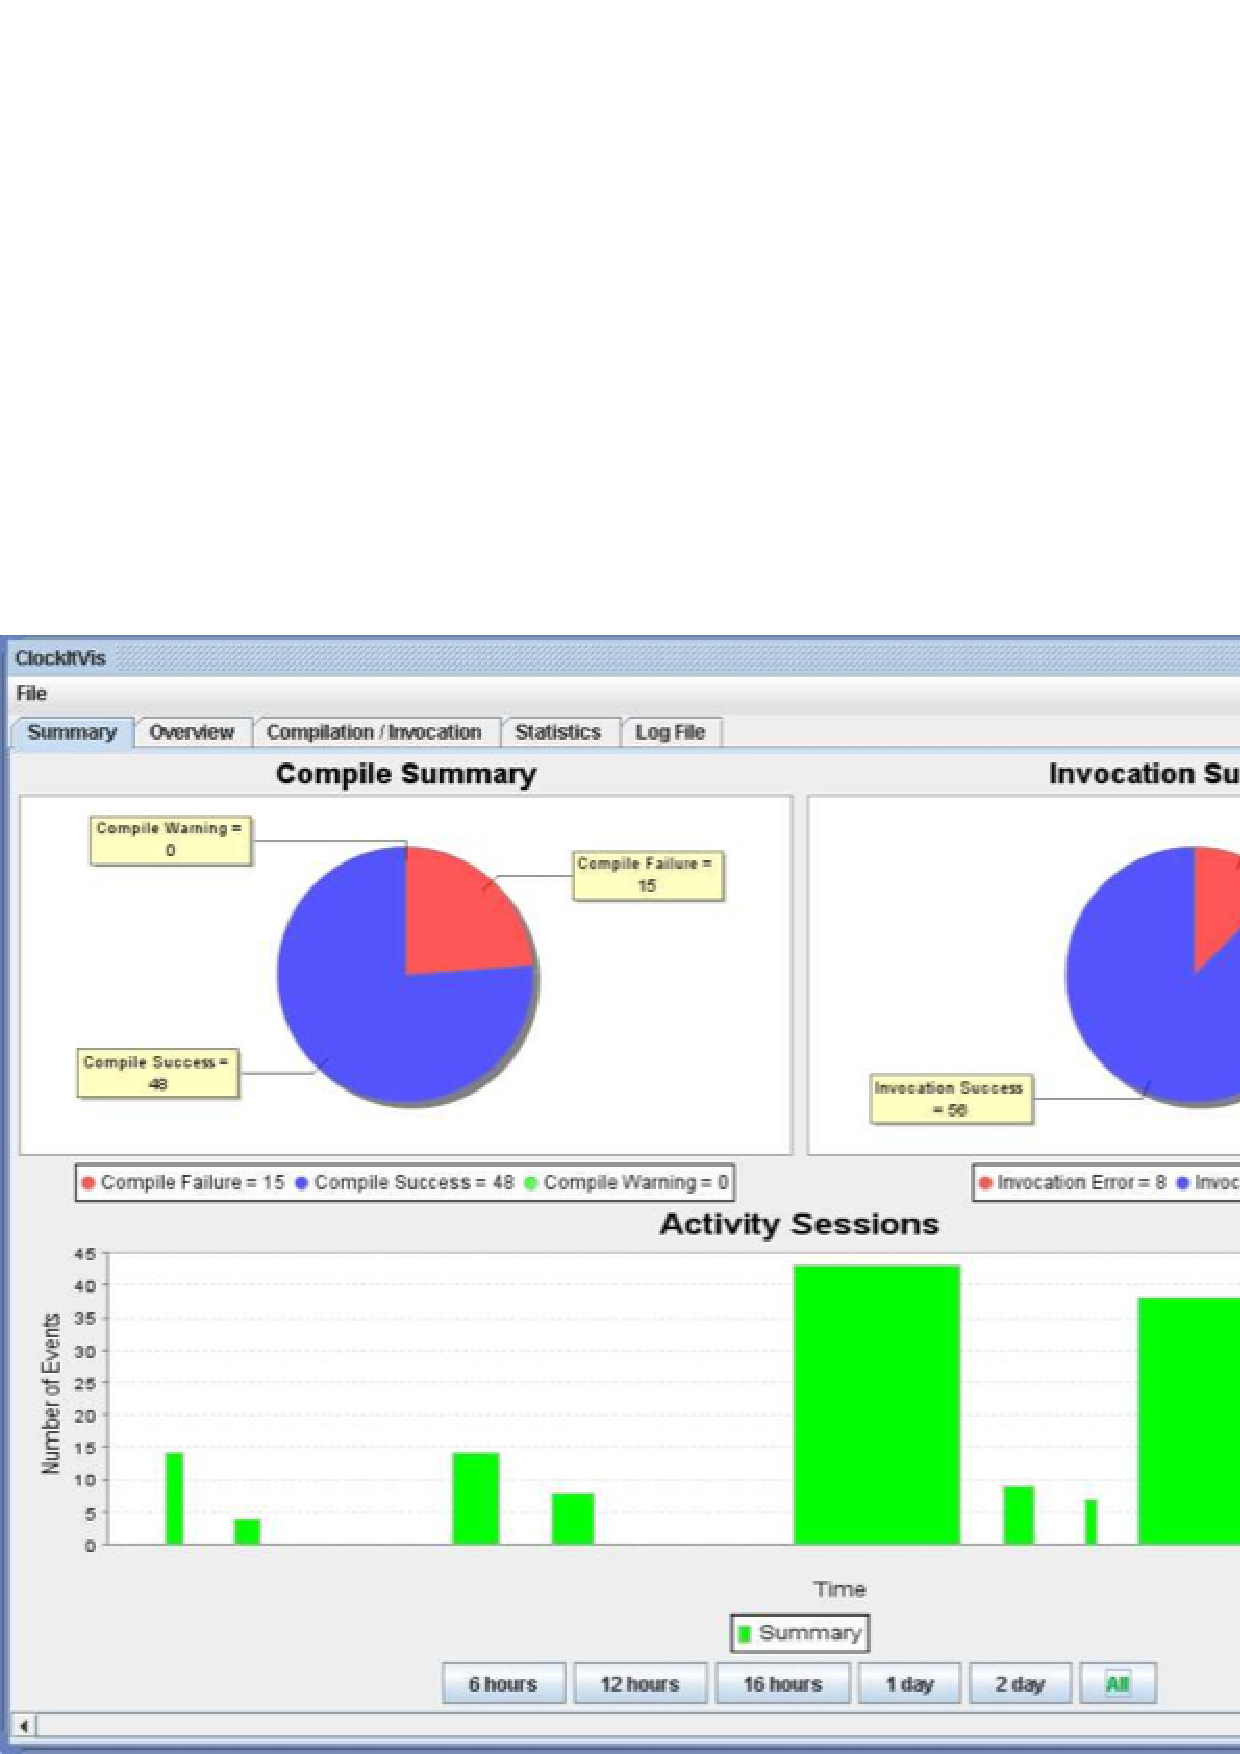
\includegraphics[height=20em]{clockit} 
   \caption{ClockIt BlueJ Data Visualizer summary}
   \label{fig:clockit}
\end{figure}

Research of Retina is closely related to ClockIt, which also provides automation data collection. Though Retina provide more tool supports (BlueJ, Eclipse and command-line compiler), it focuses on a even smaller area of programming events: the compilation. It gather data of students' compilation events, mostly compilation errors. In additional to its data viewer (see \autoref{fig:retina}), they also provide a recommendation tool for students. The tool use instant messaging (IM) to give students recommendation of approximation of amount of time one will spend on the upcoming assignment, and the compilation errors one is likely to make. These are based on both the student's previous data and the data from courses of previous semesters. 

\begin{figure}[htbp]
     \centering
     \subfigure[Retina Instructor Viewer]{
          \label{fig:retina-teacher}
          \includegraphics[width=.48\textwidth]{retina-teacher}}
     \subfigure[Retina Student Viewer]{
          \label{fig:retina-teacher}
          \includegraphics[width=.48\textwidth]{retina-student}}
          
     \caption{Data viewers of Retina.}
     \label{fig:retina}
\end{figure}

The most difference between these two research and Software ICU is that they focus only on introductory level courses, where compilation is the major interesting development event. But in other hand, their relatively easier configuration complements one of the major short-coming of Hackystat and Software ICU, which is also one of the direction we are going to improve. While neither of them provide good extensibility, they are unlikely to be useful in advantage programming situations like advantage programming course or professional setting.

PRO Metric (PROM) \cite{prom03} is the only research, to our knowledge, that is similar to Hackystat. ...

Recently, a case study of PROM in industrial environment was published\cite{prom09}. The study is based on a two year application of their PROM Experience Management system (PEM)\cite{pem08} to the IT department of a large company in Italy.

\section {Software Project Dashboards}
In software industry, there exists many commercial software project manage dashboards, such as LightHouse, ProjectManager.com dashboard, PivotLink Dashboards, Autotask Project Management and so forth. However, many of them are complete solution of software development business management, including not only software project states management, but also related resource allocation and budget control, etc. As being commercial products, they are not open source. Most importantly, there is few research published about these commercial project dashboards. ``Features'' are advertised as other commercial products, while short-comings are ignored. Thus negative results of their use are unknown. This research of Software ICU contains not only its benefits, but also its negative impact.


\section {Previous Case Studies of Hackystat}
The classroom study presented in this thesis is the third case study of Hackystat system in a classroom setting. 

The first case study is performed in 2003 using an early version of Hackystat\cite{csdl2-03-13}. During that time, Hackystat was only collecting 4 types of metrics (Active Time, Size, Unit Tests and Coverage). The system was oriented around a set of ``Course'' analyses that were tailored to an educational setting. Those analyses summaries of the individual team project metric data to-date in tabular form, and also presented comparisons of all of the course projects\autoref{fig:hackystat2003}. The evaluation shows that the installation of Ant sensors is the most significant barrier to the system. It was too difficult to install if without direct help from the development team. But the overhead of use is relatively low and analyses were usable and useful, while data privacy was uncomfortable for some students.

\begin{figure}[htbp]
   \centering
   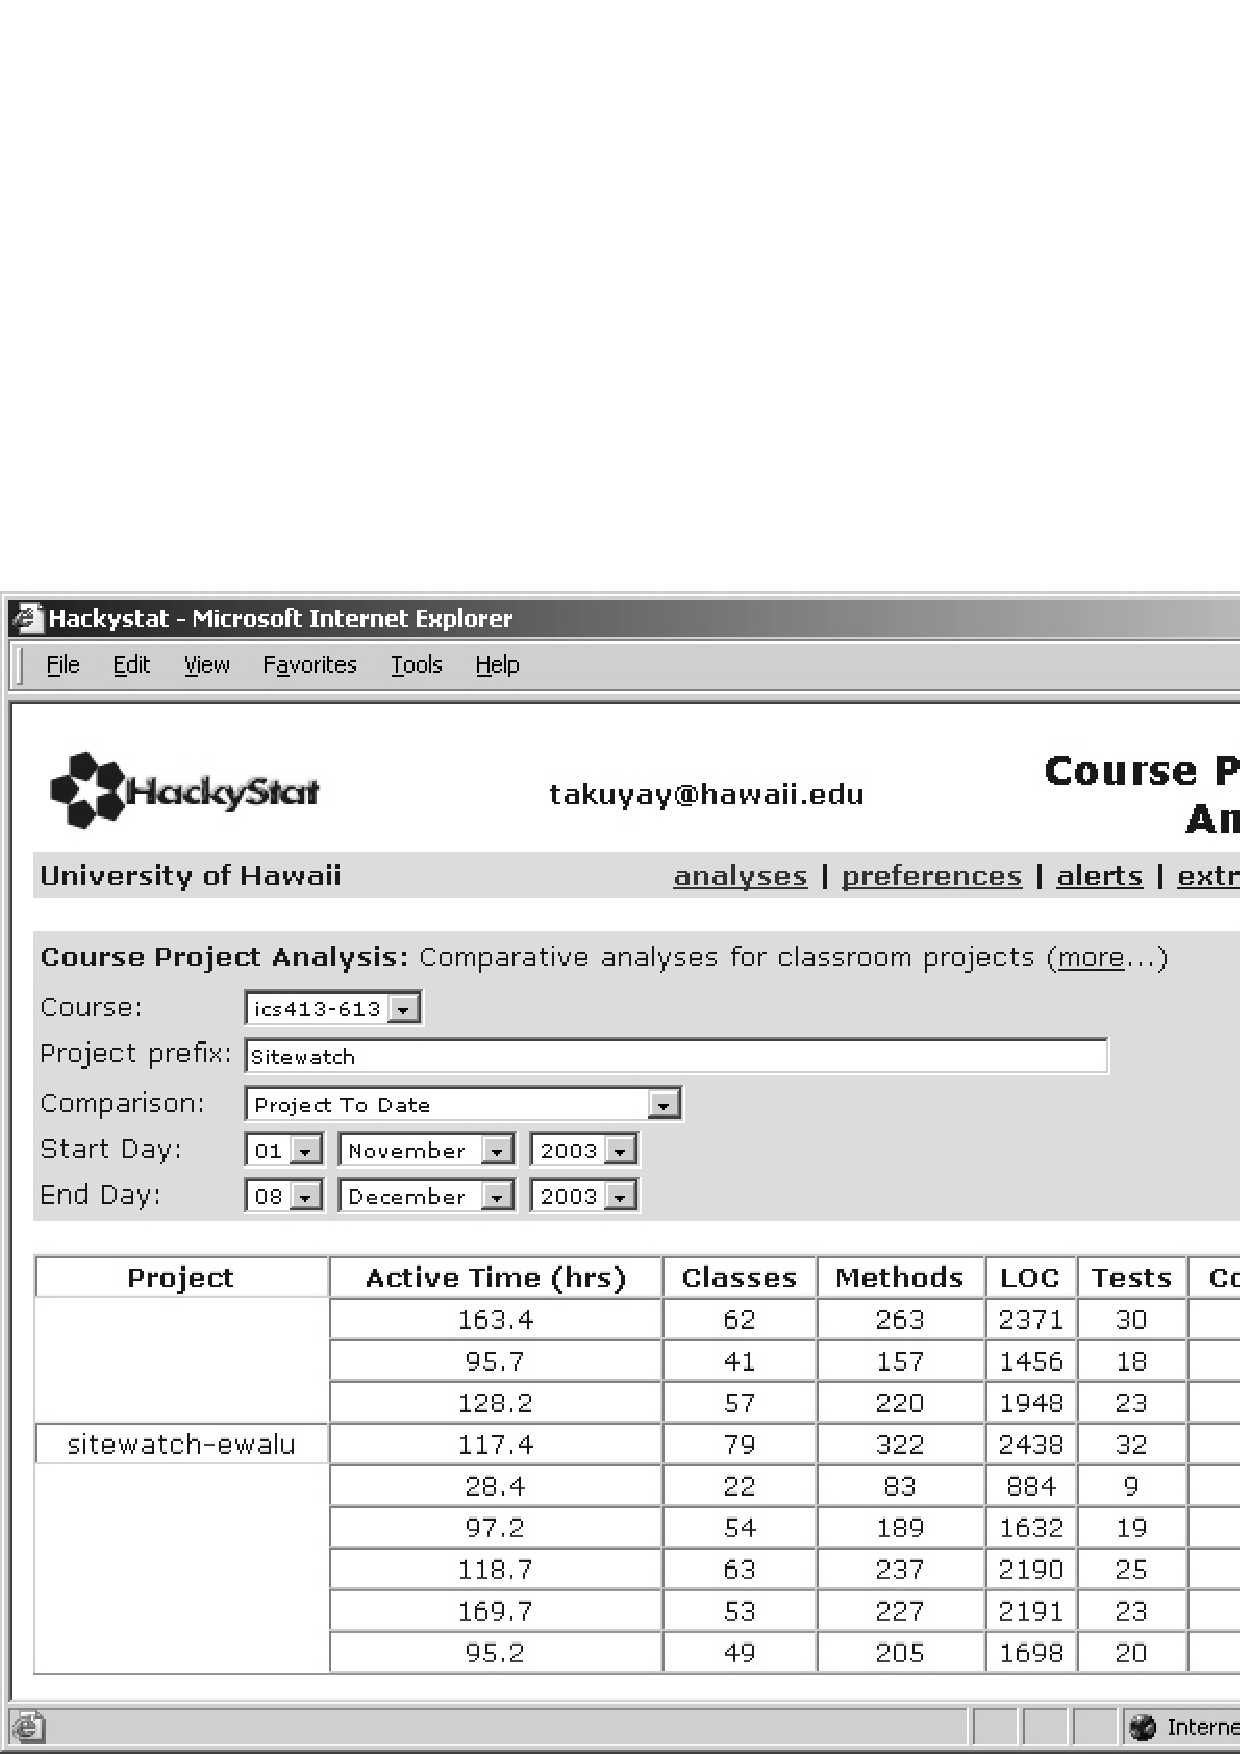
\includegraphics[height=20em]{hackystat2003} 
   \caption{Screenshot of course project to date analysis of Hackystat in 2003}
   \label{fig:hackystat2003}
\end{figure}

The second case study happened in 2006 as a partial replication of the first case study\cite{csdl2-07-02}. The Hackystat had undergone significant change from 2003 to 2006. The sensor installation, which is the major barrier to the system in 2003, was automated by the hackyInstaller GUI, which greatly lower the overhand of configuration for developers. The evaluation also shows significant drop in sensor installation difficulty. However, the new sophisticated Telemetry analysis \autoref{fig:hackystat2006} and its complex user interface raise the difficulty of using it and interpreting data, lead to slightly drop of usability and professional feasibility.

\begin{figure}[htbp]
   \centering
   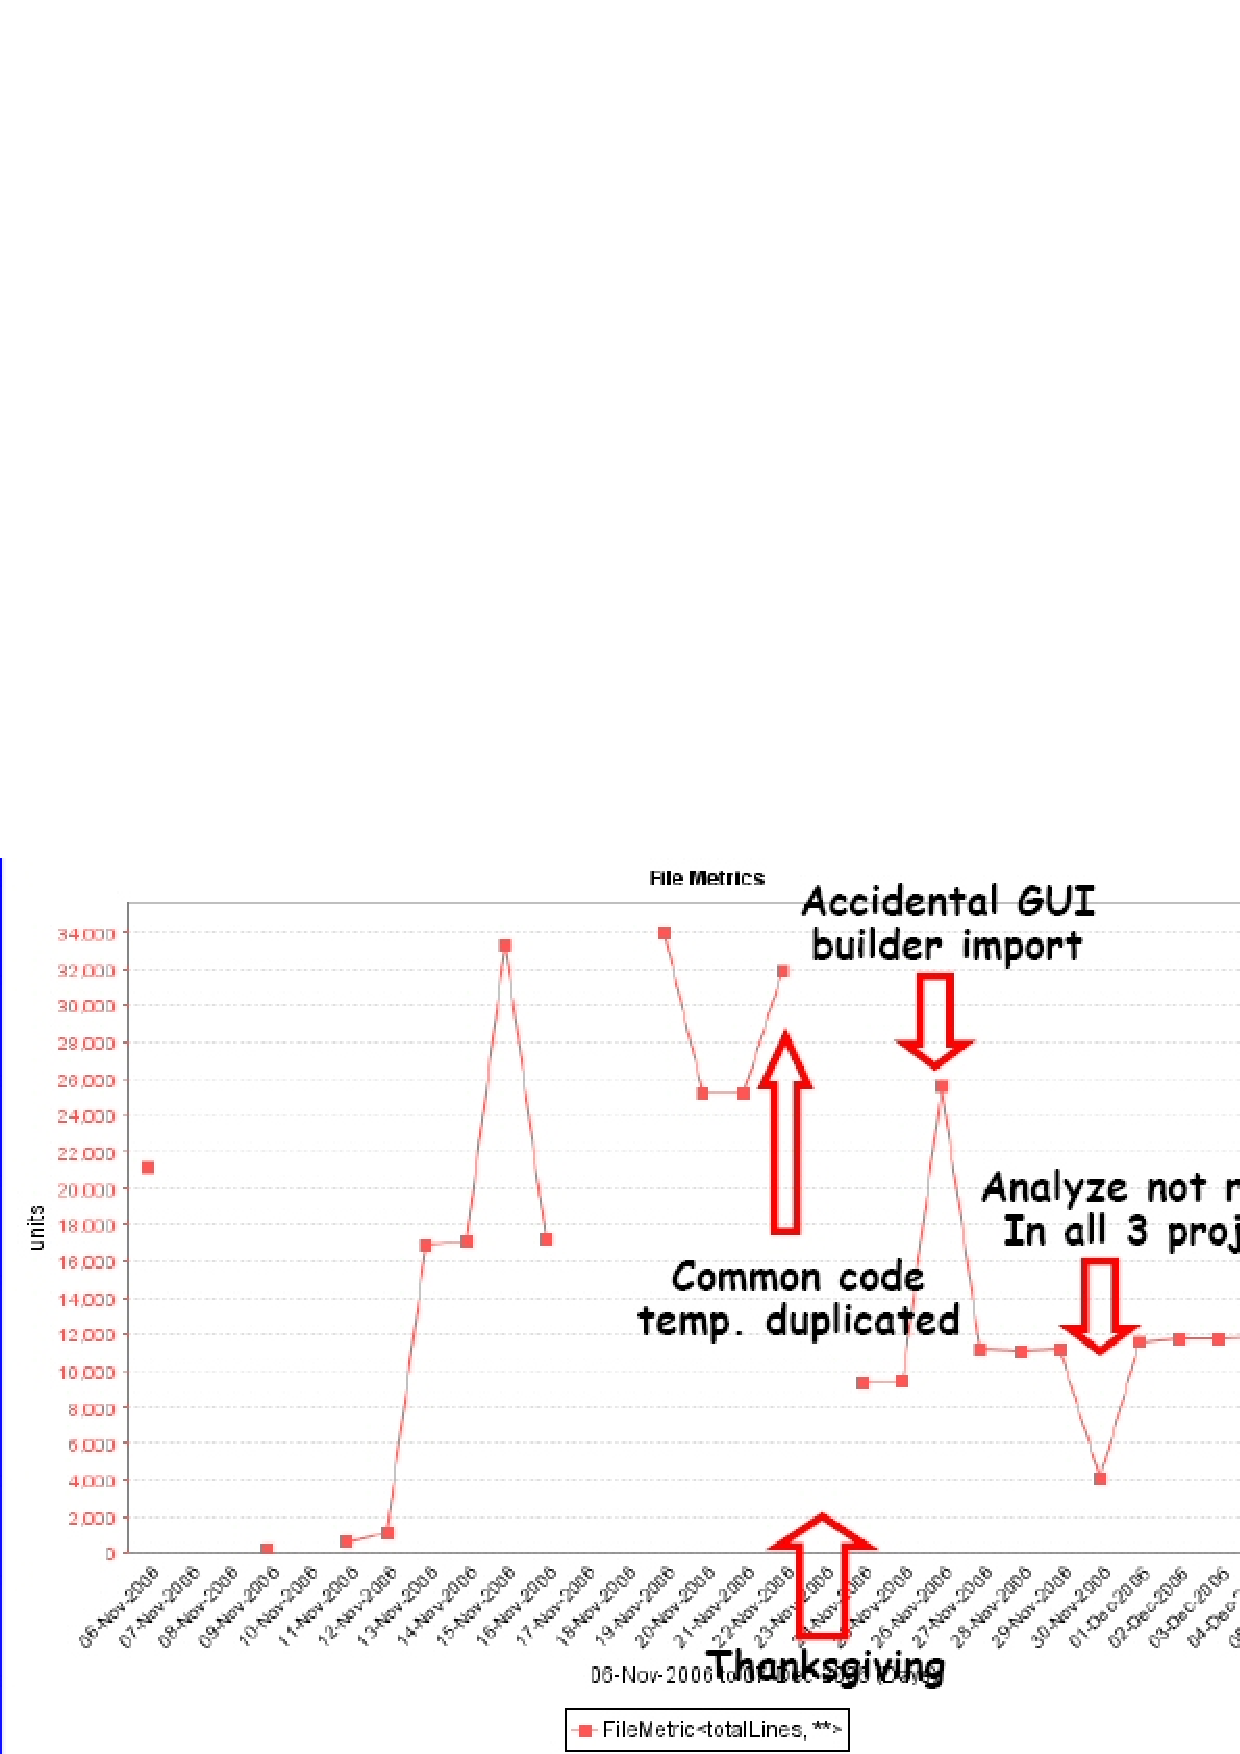
\includegraphics[height=20em]{hackystat2006} 
   \caption{Screenshot of file-metric telemetry analysis of Hackystat in 2006}
   \label{fig:hackystat2006}
\end{figure}

In 2007, Hackystat has been re-implemented to a new architecture version. Adopting the service-oriented architecture enable us to design multiple user interface separately from the kernel components. The Software ICU is built upon a new web-based UI called Project Browser, and the classroom study is also based on this user interface.


\chapter{Hackystat}
In this research, I utilize Hackystat to implement the Software ICU. This chapter briefly introduce the Hackystat system, which was invented by Professor Philip M. Johnson, in the Collaborative Software Development Laboratory, Department of Information and Computer Sciences, University of Hawaii at Manoa. 
 

\section{Hackystat Framework}
Hackystat is an open source framework for collection, analysis, visualization, interpretation, annotation, and dissemination of software development process and product data.

Hackystat users typically attach software ``sensors'' to their development tools, which unobtrusively collect and send ``raw'' data about development to a web service called the Hackystat SensorBase for storage.

The SensorBase repository can be queried by other web services to form higher level abstractions of this raw data, and/or integrate it with other internet-based communication or coordination mechanisms, and/or generate visualizations of the raw data, abstractions, or annotations.

\subsection{Daily Project Data Analysis}
The DailyProjectData(DPD) service is one of Hackystat's most important fundamental analysis service. From the raw sensor data in the SensorBase repository, it creates various abstractions of sensor data associated with a single project for a single 24 hour period, which usually represents a simple software development metric in a single day.

\subsection{Telemetry Analysis}
The Telemetry service is another fundamental analysis of Hackystat. Based on data from DPD service, it supports the creation of trend lines that show how various characteristics of software development are changing over time. To support the work practices of different organizations, it provides a domain specific language that allows the creation of custom trend lines (called telemetry "streams") and their visualization together in a specific telemetry "chart". 

Telemetry streams support various numbers of parameters. User can use them to generate more specific streams. In our Project Portfolio Analysis, which based on Telemetry service, user can configure the parameters of each Telemetry analysis. More detail will be discuss in later part.

\section {Project Browser and Wicket}
Wicket is one of the dozens of Java web frameworks, but a outstanding one. It use HTML attributes to denote components, enabling easy editing with ordinary HTML editors. The internal object structure is similar to Swing, it give easy but powerful way to develop functionality on both server and client side.

Upon it we built a web application UI to view collected data and run various analysis provided by Hackystat services, that is called Project Browser. Its goal is to simplify the usage of Hackystat service as well as provide better visualization over the analysis data.


\section {Software Intensive Care Unit}
The Software Intensive Care Unit(SICU) consist a table of metrics over each of the projects. Each metrics are shown with a spark-line and a number value, each of which will be colored conditionally. The spark-line is generated using the Google Chart API.\cite{googlechart}

\chapter{Design and Implementation of Software ICU}
\section{Software Intensive Care Unit}
In order utilize the well developed software engineering measures to achieve good management of software development projects, we introduce a system called Software Intensive Care Unit consists of a number of software development metrics and use these metrics to generate a number of vital signs that state represent "health" state of software development projects.

\section{Vital Signs}
Vital signs of software projects are measured by various software development process or product metrics. Each of these metric reveal an aspect of the state of the software project.
\begin{description}
\item[Coverage] 
Coverage is a measure used in software testing. It describes the degree to which the source code of a program has been tested. It measures the quality of the tests, which is an essential part of program quality insurance.
\item[Cyclomatic complexity] 
Cyclomatic complexity, was developed by Thomas J. McCabe and is used to measure the complexity of a program. It directly measures the number of linearly independent paths through a program's source code.\cite{mccabe:complexity} Higher cyclomatic complexity means more distinct control paths in a program module, thus it is more difficult to fully test them and the untested paths may have deficiency inside. Therefore, program modules are preferred to have lower complexity.
\item[Coupling] 
Coupling, or say dependency, is the degree to which each program module relies on each one of the other modules.\cite{wiki:coupling} It is actually a measure of the complexity of the whole system's module reference tree. Whenever one module is modified, there will be a chance that the changes may cause bugs in one of modules that relies on this one. Therefore, higher coupling value implies higher risk of introducing bugs when making changes, thus more difficult to maintain the system.
\item[Churn] 
Churn is a measure of the total number of lines of code deleted and added. It represent the amount of changes made to the system, which reflects the work to the system. Interpretation of this metric is conditional. Low churn means low work load to the system, but also means consistency of the system, thus is good for systems under maintenance. However, high churn implies higher inconsistency of the source code of the system, but also means high work load, which is the normal case of a intensively developing project.
\item[Size] 
The size of software program is measured by the source lines of code (SLOC), which counts the number of lines in the text of the program's source code. SLOC is typically used to predict the amount of effort that will be required to develop a program, as well as to estimate programming productivity or effort once the software is produced.
\item[Commit] 
Commit measure the number of commitments made to the source code repository. It is recommended that programmer should make commit often and make it small and keep the integration consistent.
\item[DevTime] 
DevTime, abbreviation of Develop Time, is a measure of total human work put into the system.
\item[Build] 
Build is a count of ant build task invoked in a period of time.
\item[Test] 
Test is a count of unit tests invoked in a period of time.
\end{description}

\subsection{Vital Sign from latest value}
Latest values of software metrics are important enough to be shown separately because they represent the latest state of a project. We assign colors to latest value of the measures to indicate their performing.

\subsection{Vital Sign from historical trend via spark-line}
Historical data of software metric is as good as the latest one. It provides more information of the performance of the project over time. But in the same time it bring a great amount of data overwhelming as well. In order to reduce the historical data to an acceptable small but meaningful degree, we use spark-line to represent them. Then we assign colors to the spark-lines with several evaluation strategies: Stream Trend and Participation.

\subsubsection{Stream Trend Evaluation}
Stream trend evaluation determines the health of a stream by its trend. It takes one parameter called HigherBetter. If user define the higher value the better, then increasing trends will be considered as a healthy trend and decreasing trends will be considered as unhealthy. Stable trends are always considered as healthy because in that case it is as good as health that one don't need to pay too much attention to it, while the actual value will be shown in the latest value where the value will be judged to be good or not. And unstable trend is marked as average because it is not easy to tell if it indicates a good state or not. 

\subsubsection{Participation Evaluation}
Participation evaluation determines the health of a stream by the participations of all members in the project. When working as a group, it is not good that some of the member do most of the work and others do little, thus in this situation the stream will be classified as unhealthy stream, which mean to attract attention.

\chapter{Classroom Evaluation}
We evaluate this system in a classroom setting. The class contain 20 students. They are learning software development methods in the class and will use the system for about a month till the end of the semester. During this period, they work as small group of 3~4 people, and each group will work on 2 software projects.

We gather research data in two ways:
	1. We will monitor and log their usage of the system. From this data we can find out their frequency and habit of using the system. And compared with their performance of the project, we can analysis the helpfulness of the system in developer's aspect. 
	2. We will give out survey at the end of the semester to gather their opinions of the system. From this we can find out users' attitude towards the system. In additional, they may provide insightful suggestion to improve the system.

We will analyze this data along with the data from previous Hackystat studies.

\chapter{Contribution and Future Directions}

\section{Current Defects}

\subsection{Data Completeness}

DevTime does not show completely the time developers spent on the project. 

Defects: Fail of unit testing and coverage does not necessary indicate the number of defects in the code. Code review data is needed. 


